\section{EiffelStudio}
EiffelStudio is a full-featured, commercial grade IDE for the Eiffel Programming Language (\cite[Quote from Origo website]{eiffel2006}). It has many tools to ease the design of systems with Eiffel and is focused on providing an ``all-in-one" package for the user, so that no outside software is needed.

\begin{figure}[h]
\centerline{
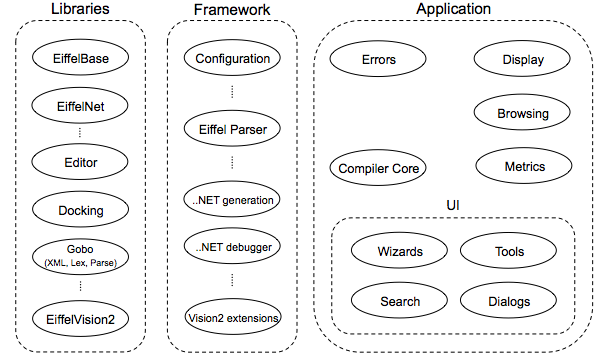
\includegraphics[scale=0.7]{images/eiffelstudio-structure-full.png}
}
\caption[Overview of the EiffelStudio structure]{Overview of the EiffelStudio structure.}
\label{fig:eiffelstudio_structure}
\end{figure}


\subsection{The system}
EiffelStudio consists of three main sections; Libraries, Framework, and Application (as seen in figure \ref{fig:eiffelstudio_structure}). This project mainly focuses on the \textsc{ui} subsection of Application, more specifically, the Tools part.

\paragraph{}
The \textsc{ui} consists of toolbars, tools and windows. The window shows the user the currently viewed context in the desired fashion, which for instance can be the pure source code or a specific perspective on the source code, but also a visual representation of it. The toolbars and tools allow the user to switch what is currently shown in the window without altering the source. When a user wants to change this, he will select the appropriate perspective, and the window will be informed by this by the bar or tool in being utilized. When displaying text, the window uses different formatters to translate the underlying source to the desired perspective on the code. The specific formatters does this by having a specialized output strategy define the text shown in the window based on an abstract Eiffel syntax. Figure \ref{fig:eiffelstudio_view_change} shows an overview of this. This is a description of how this works conceptually, and therefore might differ slightly from the actual implementation. A more precise description can be found in section \ref{implementation_eiffelstudio}

\begin{figure}[H]
\centerline{
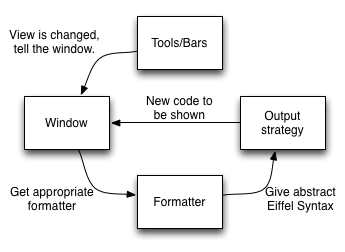
\includegraphics[scale=0.7]{images/eiffel_view_text_design.png}
}
\caption[EiffelStudio view control]{Overview of how EiffelStudio changes views.}
\label{fig:eiffelstudio_view_change}
\end{figure}

\subsubsection{Why in a view?}
\label{why_a_view}
EiffelStudio has multiple ways of showing different perspectives on the same code. This is done by the View feature which allows for switching between perspectives, or views. While viewing a piece of Eiffel source code, the user can switch to the interface view, for instance, where you can see the signature, comments and contracts of all the features  of the current class, including inherited ones. This gives the user the ability to overview over the structure of the class, through showing information not normally available, and hiding information that is not relevant to the view. In the case of the interface view, the body of features is hidden to ensure a proper overview and to remove clutter from viewing too many features at once.
\paragraph{}
The function of the textual \textsc{bon} tool is similar to this in many ways. The tool allows the user to see the code from a textual \textsc{bon} perspective, where the idea of charts (informal) and components (formal) to help creating an overview over the structure of the code. The exact functionality of the \textsc{bon} tool will be discussed in later sections. Due to the similarity between the currently implemented views and the textual \textsc{bon} tool, adding the new tool as a view makes it feel like an integrated part of EiffelStudio, and not some external tool.

\subsection{BON syntax highlighting}